\section{Water Systems }\label{water-systems}

Water systems include a variety of components that simulate water consumption, production, and storage, including:

\begin{enumerate}
\item Water Use Equipment and Connections
\item Rainwater Collection
\item Groundwater Well
\item Water Storage Tanks
\end{enumerate}

\subsection{Water Mains Temperatures}\label{water-mains-temperatures}

The input object Site:WaterMainsTemperature provides a model for the temperature of water mains that deliver water to a building via underground pipes.~ The water mains temperatures are an important input for plant equipment that require make-up water from the water mains, such as for domestic hot water systems.

Water mains temperatures are a function of outdoor climate conditions and vary with time of year.~ A correlation has been formulated to predict water mains temperatures based on two weather inputs:

\begin{itemize}
\item average annual outdoor air temperature (dry-bulb)
\item maximum difference in monthly average outdoor air temperatures
\end{itemize}

These values can be easily calculated from annual weather data using a spreadsheet.

The correlation was developed by Craig Christensen and Jay Burch and is described in Hendron et al. (2004).~ The correlation is:

\begin{equation}
T_{mains} = (T_{out,avg} + 6) + ratio * (\Delta T_{out,maxdiff} / 2) * SIN(0.986 * (day - 15 - lag) - 90)
\end{equation}

where:

T\(T_{mains}\) is the water mains temperature (\(^{\circ}\)F)

T\(T_{out,avg}\) is the average annual outdoor air temperature (\(^{\circ}\)F)

\({\Delta T_{out,maxdiff}}\) is the maximum difference in monthly average outdoor air temperatures (\(^{\circ}\)F)

day is Julian day of the year (1-365)

ratio is equal to 0.4 + 0.01 * (Tamb,avg - 44)

lag is equal to 35 - 1.0 * (Tamb,avg - 44) (\(^{\circ}\)F).

For the Chicago-O'Hare TMY2 weather file, \(T_{out,avg}\) = 9.69\(^{\circ}\)C and \({\Delta T_{out,maxdiff}}\) = 28.1\(^{\circ}\)C.~ The resulting water mains temperature profile is graphed in Figure~\ref{fig:water-mains-temperatures-chicago-ohare-TMY2}.

\begin{figure}[htbp]
\centering
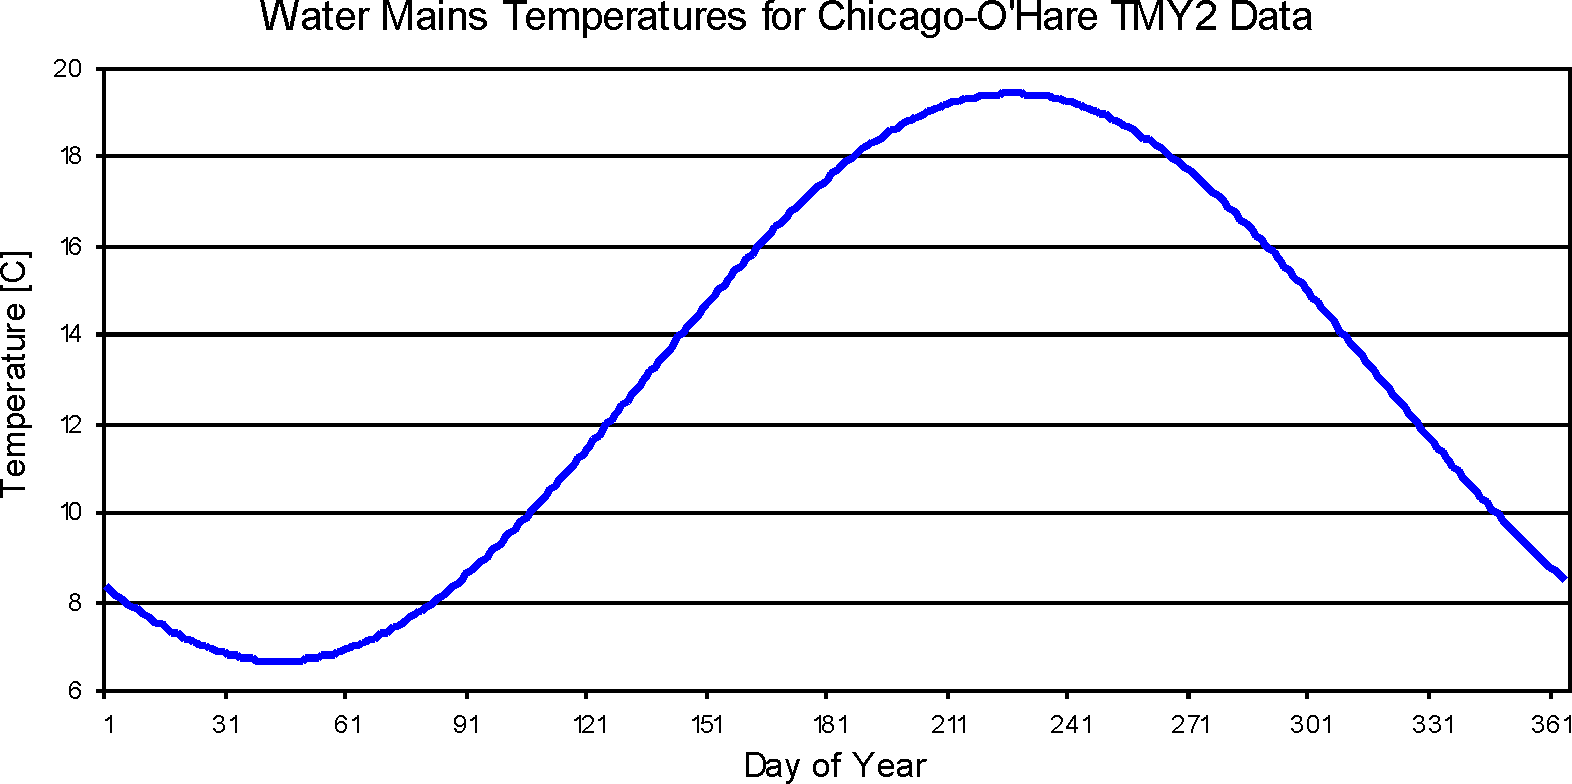
\includegraphics{media/image6936.png}
\caption{Water Mains Temperatures for Chicago-O'Hare TMY2 Data \protect \label{fig:water-mains-temperatures-chicago-ohare-TMY2}}
\end{figure}

\subsubsection{References}\label{references-052}

Hendron, R., Anderson, R., Christensen, C., Eastment, M., and Reeves, P.~ 2004.~ ``Development of an Energy Savings Benchmark for All Residential End-Uses'', Proceedings of SimBuild 2004, IBPSA-USA National Conference, Boulder, CO, August 4 - 6, 2004.

\subsection{Water Use Equipment and Connections}\label{water-use-equipment-and-connections}

Essential parts of most water systems are the end uses where the water is utilized for a purpose.~ These end uses are characterized by familiar pieces of equipment such as sinks, showers, dishwashers, clothes washers, and toilets.~ End uses can also include outdoor uses such as landscape irrigation and agricultural irrigation.

Water end-use modeling in EnergyPlus is accomplished via two input objects:

\begin{itemize}
\item WaterUse:Equipment
\item WaterUse:Connections
\end{itemize}

The WaterUse:Equipment object simulates all different types of water end uses.~ The WaterUse:Connections object manages multiple pieces of water equipment with a common supply and return, internally providing the services of a splitter and a mixer.~ The WaterUse:Connections object also allows water consuming equipment to be simulated in a closed plant loop by supplying makeup water from the water mains.

\subsection{Unconnected Water Use Equipment}\label{unconnected-water-use-equipment}

Common water equipment, such as sinks and showers, requires mixing of hot and cold water to provide a desired temperature at the tap.~ Water use equipment that is simulated in ``unconnected'' mode, i.e., without being referenced by a WaterUse:Connections object, presents a relatively simple modeling problem illustrated in Figure~\ref{fig:hot-and-cold-water-mixing}.

\begin{figure}[hbtp] % fig 315
\centering
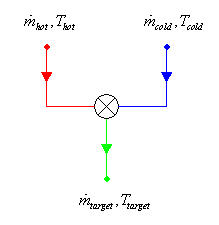
\includegraphics[width=0.9\textwidth, height=0.9\textheight, keepaspectratio=true]{media/image6937.png}
\caption{Hot and Cold Water Mixing \protect \label{fig:hot-and-cold-water-mixing}}
\end{figure}

The variables are defined as:

\({\dot m_{hot}}\) is the hot water supply mass flow rate

\({T_{hot}}\) is the hot water supply temperature

\({\dot m_{cold}}\) is the cold water supply mass flow rate

\({T_{cold}}\) is the cold water supply temperature

\({\dot m_{target}}\) is the target mass flow rate at the tap

\({T_{target}}\) is the target temperature at the tap.

The basic physics of the problem are described by two equations representing conservation of mass and conservation of energy respectively:

\begin{equation}
{\dot m_{target}} = {\dot m_{hot}} + {\dot m_{cold}}
\end{equation}

\begin{equation}
{\dot m_{target}}{T_{target}} = {\dot m_{hot}}{T_{hot}} + {\dot m_{cold}}{T_{cold}}
\end{equation}

The hot and cold water supply temperatures, \({T_{hot}}\) and \({T_{cold}}\), are specified by the user with schedules (or indirectly from the water mains temperatures).~ The target flow rate and target temperature, \({\dot m_{target}}\) and \({T_{target}}\), at the tap are also specified with schedules.~ The target conditions can be thought of as a way to simulate occupant behavior; a person at a sink will adjust the hot and cold flow rates to get the overall water flow and temperature that is desired.

The two equations above are easily solved to calculate the necessary hot and cold flow rates needed to attain the target conditions.

\begin{equation}
{\dot m_{hot}} = {\dot m_{target}}\left( {\frac{{{T_{target}} - {T_{cold}}}}{{{T_{hot}} - {T_{cold}}}}} \right)
\end{equation}

\begin{equation}
{\dot m_{cold}} = {\dot m_{target}} - {\dot m_{hot}}
\end{equation}

Even though hot and cold flow rates are unlimited in ``unconnected'' mode, it is still possible to fail to meet the target conditions if \({T_{target}}\) ~\textgreater{} \({T_{hot}}\).~ In this case, the actual mixed water temperature at the tap, \({T_{mixed}}\), is set equal to \({T_{hot}}\).~ The target flow rate is always met.

Water equipment that omits schedules for the target temperature and/or hot water supply temperature implies that no hot water is needed.~ The result is all cold water at the target flow rate.

For ``unconnected'' water equipment, the heating rate and energy that is required to supply the hot water is calculated by the following equations.

\begin{equation}
Q = {\dot m_{hot}}{c_p}\left( {{T_{hot}} - {T_{cold}}} \right)
\end{equation}

\begin{equation}
\Delta E = Q\Delta t
\end{equation}

where:

\(Q\) is the heating rate

\({c_p}\) is the specific heat of water

\(\Delta E\) is the heating energy

\(\Delta t\) is the time step interval.

All heating is assigned to ``Purchased Heating''.

\subsection{Zone Heat Gain from Water Use Equipment}\label{zone-heat-gain-from-water-use-equipment}

Some water use equipment can be a significant source of sensible and latent heat gain when located in a zone.~ Showers, for example, add a noticeable latent gain as some of the hot water evaporates into the zone air (and at the same time adding some sensible gain).~ Other types of equipment may contribute greater sensible gain but less latent gain.

Calculating the amount of sensible and latent heat gain can be extremely complicated and depends on many variables.~ One set of variables is related to the initial conditions of the entering water and the undisturbed zone air, namely:

\begin{itemize}
\item
  Entering water temperature
\item
  Entering water flow rate
\item
  Ambient zone air temperature
\item
  Ambient zone humidity
\item
  Ambient zone barometric pressure
\end{itemize}

A second set of variables is tied to the specifics of the water equipment which describe the heat and mass transfer processes that occur as the water passes through the zone.~ These variables might include the velocity of the water in the zone air, the surface area of water exposed to the zone air, the dwell time of water in the zone, and possibly others.~ The complexity of these variables cannot be easily cast into a generalized EnergyPlus input object.~ Consider that in a shower, the velocity of water droplets is increasing as they fall, and the surface area of the spray is increasing.~ How does one even determine the surface area of the spray at any point?

The approach taken here is to utilize the first set of initial condition variables and forego the overly-complex second set.~ The initial conditions can be used to calculate a maximum possible change in sensible and latent energy between the entering water conditions and the leaving water conditions at an infinite time later.~ Sensible and latent energy are calculated separately and represent the maximum heat gain, respectively, that could be added to the zone air.~ The user simply specifies a fraction of the maximum heat gain for sensible and latent that is actually added to the zone air.~ The fraction is specified with a schedule to account for different modes of operation.~ The split between sensible and latent will vary depending on the type of equipment that is to be modeled.~ Typically, both fractions should be small numbers.

\begin{figure}[hbtp] % fig 316
\centering
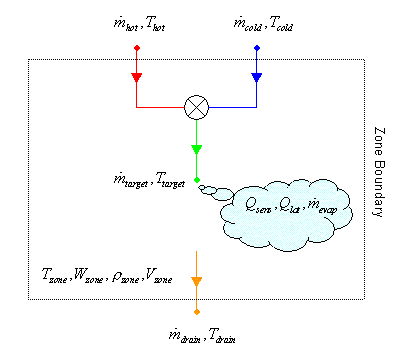
\includegraphics[width=0.9\textwidth, height=0.9\textheight, keepaspectratio=true]{media/image6962.png}
\caption{Zone Heat Gain from Water Use Equipment \protect \label{fig:zone-heat-gain-from-water-use-equipment}}
\end{figure}

The maximum sensible heat gain rate is calculated by assuming that all of the water flow is allowed to cool to the zone dry-bulb temperature.~ The actual sensible zone heat gain rate is found by multiplying the maximum by the user fraction.

\begin{equation}
{Q_{sens}} = {f_{sens}}{\dot m_{target}}{c_p}\left( {{T_{target}} - {T_{zone}}} \right)
\end{equation}

\begin{equation}
\Delta {E_{sens}} = {Q_{sens}}\Delta t
\end{equation}

where:

\({Q_{sens}}\) is the sensible heat gain rate

\({f_{sens}}\) is the user fraction of maximum sensible heat

\({\dot m_{target}}\) is the target mass flow rate at the tap

\({c_p}\) is the specific heat of water

\({T_{target}}\) is the target temperature at the tap

\({T_{zone}}\) is the zone dry-bulb air temperature

\(\Delta {E_{sens}}\) is the sensible heat gain

\(\Delta t\) is the time step interval.

The maximum latent heat gain rate is calculated by assuming that the maximum amount of water is evaporated into the zone air during the time step.~ The actual latent zone heat gain rate is found by multiplying the maximum by the user fraction.

\begin{equation}
{m_{evap,zonemax}} = \left( {{W_{sat}} - {W_{zone}}} \right){\rho_{zone}}{V_{zone}}
\end{equation}

\begin{equation}
{m_{evap,flowmax}} = {\dot m_{target}}\Delta t
\end{equation}

\begin{equation}
{m_{evap,max}} = MIN({m_{evap,zonemax}},{m_{evap,flowmax}})
\end{equation}

\begin{equation}
{m_{evap}} = {f_{lat}}{m_{evap,max}}
\end{equation}

\begin{equation}
{\dot m_{evap}} = {m_{evap}}/\Delta t
\end{equation}

\begin{equation}
{Q_{lat}} = {h_{fg}}{\dot m_{evap}}
\end{equation}

\begin{equation}
\Delta {E_{lat}} = {Q_{lat}}\Delta t
\end{equation}

where:

\({m_{evap,zonemax}}\) is the mass of water that can be absorbed by the zone air in one timestep

\({W_{sat}}\) is the fully-saturated zone humidity ratio (function of air temperature and pressure)

\({W_{zone}}\) is the zone humidity ratio

\({\rho_{zone}}\) is the zone dry-air density (function of air temperature and pressure)

\({V_{zone}}\) is the zone air volume

\({m_{evap,flowmax}}\) is the mass of water available in the flow in one timestep

\({\dot m_{target}}\) is the target mass flow rate at the tap

\(\Delta t\) is the time step interval

\({m_{evap,max}}\) is the maximum mass of water that can be evaporated

\({m_{evap}}\) is the actual mass of water evaporated into the zone air

\({f_{lat}}\) is the user fraction of maximum latent heat

\({\dot m_{evap}}\) is the mass rate of water evaporation into the zone air

\({Q_{lat}}\) is the latent heat gain rate

\({h_{fg}}\) is the heat of vaporization for water

\(\Delta {E_{lat}}\) is the latent heat gain.

Sensible and latent heat gains to the zone are lagged by one zone time step.

Note that this method allows the heat gain to vary dynamically according to changing water and zone conditions instead of the fixed or scheduled value that is traditionally used.~ However, sensible and latent fractions may be difficult to estimate.~ Experimental measurement is probably the best way to determine the fractions.

A related result of any zone heat and moisture gain is that the water undergoes an equal heat and moisture loss.~ For a shower the water will generally leave the zone at a cooler temperature and slightly reduced flow rate when compared to the entering water conditions.

\begin{equation}
{\dot m_{drain}} = {\dot m_{target}} - {\dot m_{evap}}
\end{equation}

\begin{equation}
{T_{drain}} = \frac{{{{\dot m}_{target}}{c_p}{T_{target}} - {Q_{sens}} - {Q_{lat}}}}{{{{\dot m}_{drain}}{c_p}}}
\end{equation}

where:

\({\dot m_{drain}}\) is the drainwater mass flow rate at the drain

\({\dot m_{target}}\) is the target mass flow rate at the tap

\({\dot m_{evap}}\) is the mass rate of water evaporation into the zone air

\({T_{drain}}\) is the water temperature at the drain

\({c_p}\) is the specific heat of water

\({T_{target}}\) is the target temperature at the tap

\({Q_{sens}}\) is the sensible heat gain rate

\({Q_{lat}}\) is the latent heat gain rate.

The change in leaving water conditions has implications for drainwater heat recovery and storage tank conditions.

\subsection{Connected Water Use Equipment}\label{connected-water-use-equipment}

Water use equipment referenced by a WaterUse:Connections object is considered to be in ``connected'' mode.~ The WaterUse:Connections object manages multiple pieces of water equipment with a common supply and return, internally providing the services of a splitter and a mixer.~ The connections object also offers three internal configurations for drainwater heat recovery.~ External connections are available for coupling to plant loop nodes or water storage tanks for graywater reuse or reclamation.

Keep in mind that water use equipment in ``connected'' mode does not imply that it is connected to a plant loop.~ WaterUse:Equipment objects are never directly connected to a plant loop; they are connected indirectly through the WaterUse:Connections object.~ WaterUse:Connections can operate either within a plant loop or in stand-alone mode, i.e., without plant loop connections.

The WaterUse:Connections object overrides the hot and cold water supply temperatures of its subordinate WaterUse:Equipment objects based on the specified schedules, plant loop conditions, or water storage tank conditions.~ But the WaterUse:Equipment objects still maintain their individual target flow rates and target temperatures.

Solving the water subsystem described by the WaterUse:Connections object is appreciably more difficult than solving a single, unconnected piece of water use equipment.~ The subsystem is illustrated in Figure~\ref{fig:water-use-connections-subsystem}.

\begin{figure}[hbtp] % fig 317
\centering

\includegraphics[width=0.9\textwidth, height=0.9\textheight, keepaspectratio=true]{media/image7005.png}
\caption{Water Use Connections Subsystem \protect \label{fig:water-use-connections-subsystem}}
\end{figure}

The nomenclature here uses uppercase letters to indicate variables related to the connections object and lowercase letters to indicate variables related to the equipment objects.~ The variables are defined as:

\({\dot M_{hot}}\) is the hot water supply mass flow rate

\({T_{hot}}\) is the hot water supply temperature

\({\dot M_{cold}}\) is the cold water supply mass flow rate

\({T_{cold}}\) is the cold water supply temperature

\({\dot M_{drain}}\) is the drainwater mass flow rate at the drain

\({T_{drain}}\) is the water temperature at the drain

\({T_{waste}}\) is the wastewater temperature after the drain

\({\dot M_{return}}\) is the return water mass flow rate back to the plant loop

\({T_{return}}\) is the return temperature of makeup water back to the plant loop.

\subsection{Water Use Equipment Calculations}\label{water-use-equipment-calculations}

The solution method proceeds in steps:

\begin{itemize}
\item Initialize Connections Temperatures
\item Calculate Connections Flow Rates
\item Calculate Connections Drain Temperature
\item Update Connections Nodes
\end{itemize}

\subsubsection{Initialize Connections Temperatures}\label{initialize-connections-temperatures}

Initializes the hot and cold supply water temperatures, \({T_{hot}}\) and \({T_{cold}}\), for the common supply to all the equipment.~ If plant-coupled, \({T_{hot}}\) is taken from the plant loop inlet node.~ If stand-alone, \({T_{hot}}\) is taken from the schedule.

\({T_{cold}}\) is taken from the supply water storage tank, if specified.~ Otherwise \({T_{cold}}\) is taken from the schedule.~ If a schedule is not specified, \({T_{cold}}\) is taken from the water mains.

\subsubsection{Calculate Connections Flow Rates}\label{calculate-connections-flow-rates}

First calls on each piece of equipment to simulate itself with the given supply water temperatures \({T_{hot}}\) and \({T_{cold}}\).~ The desired hot and cold flow rates for \({\dot m_{hot,i}}\) and \({\dot m_{cold,i}}\) are calculated (as described earlier) and passed back to the connections object.~ The total flow rates for \({\dot M_{hot}}\) and \({\dot M_{cold}}\) are then calculated:

\begin{equation}
{\dot M_{hot}} = \mathop \sum \limits_i {\dot m_{hot,i}}
\end{equation}

\begin{equation}
{\dot M_{cold}} = \mathop \sum \limits_i {\dot m_{cold,i}}
\end{equation}

If plant-coupled, \({\dot M_{hot}}\) is compared to the maximum flow rate available in the plant loop (after the first HVAC iteration).~ If \({\dot M_{hot}}\) ~\textgreater{} \({\dot M_{hot,max}}\), the actual flow rate is reset to equal the maximum: \({\dot M_{hot}}\) = \({\dot M_{hot,max}}\).~ New hot and cold flow rates, \({\dot m'_{hot,i}}\) and \({\dot m'_{cold,i}}\), at the equipment level are then recalculated, decreasing the hot flow rate and increasing the cold flow rate in order to still meet the target flow rate.

\begin{equation}
\alpha  = \frac{{{{\dot M}_{hot,max}}}}{{{{\dot M}_{hot}}}}
\end{equation}

\begin{equation}
{\dot m'_{hot,i}} = \alpha {\dot m_{hot,i}}
\end{equation}

\begin{equation}
{\dot m'_{cold,i}} = {\dot m_{target,i}} - {\dot m'_{hot,i}}
\end{equation}

A new mixed water temperature is also recalculated at the equipment level.

Although water storage tanks can also have a maximum flow rate on the cold side, the cold flow rate is not limited in this implementation.

\subsubsection{Calculate Connections Drain Temperature}\label{calculate-connections-drain-temperature}

At this point zone heat gains are calculated for all equipment in zones.~ The final drainwater temperatures and flow rates are determined for each piece of equipment by subtracting the lost heat and moisture (see above).~ The total drainwater temperature and flow rate for the subsystem are calculated:

\begin{equation}
{\dot M_{drain}} = \mathop \sum \limits_i {\dot m_{drain,i}}
\end{equation}

\begin{equation}
{T_{drain}} = \frac{{\mathop \sum \limits_i {{\dot m}_{drain,i}}{t_{drain,i}}}}{{{{\dot M}_{drain}}}}
\end{equation}

In the case of no drainwater heat recovery, the subsystem wastewater temperature, \({T_{waste}}\), is equal to the drainwater temperature, \({T_{drain}}\).~ (For drainwater heat recovery, see below.)~ The wastewater temperature and flow rate are propagated to the reclamation water storage tank, if specified.

\subsubsection{Update Connections Nodes}\label{update-connections-nodes}

Finally, if plant-coupled, the return water temperature, \({T_{return}}\), is passed on to the plant outlet node.~ \({T_{return}}\) is taken from the cold water supply schedule or the water mains.~ The return flow rate is equal to the hot water supply flow rate in order to preserve a closed plant loop: \({\dot M_{return}}\) = \({\dot M_{hot}}\).

For ``connected'' water equipment, the heating rate and energy that is required to supply the hot water for individual water equipment is calculated by the following equations.

\begin{equation}
Q = {\dot m_{hot}}{c_p}\left( {{T_{hot}} - {T_{return}}} \right)
\end{equation}

\begin{equation}
\Delta E = Q\Delta t
\end{equation}

where:

\(Q\) is the heating rate

\({c_p}\) is the specific heat of water

\(\Delta E\) is the heating energy

\(\Delta t\) is the time interval.

The heating rate and energy for the WaterUse:Connections is the sum of the values for its constituent water equipment objects.~ If the WaterUse:Connections object is stand-alone, all heating is assigned to ``Purchased Heating'' by the individual water equipment objects.~ If the WaterUse:Connections object is coupled to a plant loop, all heating is supplied by the plant loop equipment.

\subsection{Drainwater Heat Recovery}\label{drainwater-heat-recovery}

Drainwater heat recovery adds one more complication to the water connections subsystem.~ A heat exchanger is added between the drain and the waste outlet to recover some heat from the water before it leaves the system.~ The heat is usually recovered by preheating the incoming makeup water from the mains.

The heat exchanger can be modeled as ``ideal'', ``counterflow'', or ``crossflow''.~ One common type of drainwater heat exchanger is the gravity-film exchanger (GFX).~ The GFX can be approximated with a counterflow heat exchanger.

The destination of the preheated makeup water can be plumbed in three possible configurations:~ ``plant'', ``equipment'', ``plant and equipment''.~ In the ``plant'' configuration, all preheated water flow is returned to the plant loop to match the makeup water for the hot water supply flow.~ In the ``equipment'' configuration, all preheated water flow is directed internally within the WaterUse:Connections object to provide the makeup water for the cold water supply flow for the local water use equipment.~ In the ``plant and equipment'' configuration, the preheated water is split between both of the previous configurations.~ This is the only configuration where the flow rate is equal on both sides of the heat exchanger.

\begin{figure}[hbtp] % fig 318
\centering

\includegraphics[width=0.9\textwidth, height=0.9\textheight, keepaspectratio=true]{media/image7054.png}
\caption{Water Use Connections Subsystem with Drainwater Heat Recovery \protect \label{fig:water-use-connections-subsystem-with}}
\end{figure}

The new variables added here are defined as:

\({\dot M_{recovery}}\) is the makeup water mass flow rate in the heat exchanger

\({T_{recovery}}\) is the water temperature leaving the heat exchanger

\({T_{makeup}}\) =is the cold makeup water temperature supplied to various flows.

Another step is inserted into the solution method:

\begin{itemize}
\item Initialize Connections Temperatures
\item Calculate Connections Flow Rates
\item Calculate Connections Drain Temperature
\item Update Connections Nodes
\item \textbf{\emph{Calculate Connections Heat Recovery}}
\item Update Connections Nodes
\end{itemize}

For the ``equipment'' and ``plant and equipment'' configurations, the solution requires iteration to solve because the preheated water leaving the heat exchanger is connected to the cold water supply water, creating a feedback loop.

\subsubsection{Calculate Connections Heat Recovery}\label{calculate-connections-heat-recovery}

Based on the selected configuration, the flow rate through the heat exchanger is first determined.~ For the ``plant'' configuration, \({\dot M_{recovery}} = {\dot M_{hot}}\).~ For the ``equipment'' configuration, \({\dot M_{recovery}} = {\dot M_{cold}}\).~ For the ``plant and equipment'' configuration, \({\dot M_{recovery}} = {\dot M_{hot}} + {\dot M_{cold}}\).

The heat capacity rates on both sides of the heat exchanger are calculated and the minimum and maximum heat capacity rates, \({C_{min}}\) and \({C_{max}}\), are determined.

\begin{equation}
{C_{drain}} = {\dot M_{drain}}{c_p}
\end{equation}

\begin{equation}
{C_{recovery}} = {\dot M_{recovery}}{c_p}
\end{equation}

\begin{equation}
{C_{min}} = MIN({C_{drain}},{C_{recovery}})
\end{equation}

\begin{equation}
{C_{max}} = MAX({C_{drain}},{C_{recovery}})
\end{equation}

\begin{equation}
{R_c} = \frac{{{C_{min}}}}{{{C_{max}}}}
\end{equation}

where \({R_c}\) is the heat capacity ratio.

The effectiveness \(\varepsilon\) is then calculated for the given type of heat exchanger.~ For the ``ideal'' heat exchanger, \(\varepsilon = 1\).

For the ``counterflow'' and ``crossflow'' heat exchangers, the effectiveness is calculated using the effectiveness-NTU method, where:

\begin{equation}
NTU = \frac{{UA}}{{{C_{min}}}}
\end{equation}

For the ``counterflow'' heat exchanger:

\begin{equation}
\varepsilon = \frac{{NTU}}{{1 + NTU}},~if~{R_c}~=~1
\end{equation}

\begin{equation}
\varepsilon = \frac{{1 - EXP\left( { - NTU\left( {1 - {R_c}} \right)} \right)}}{{1 - {R_c}EXP\left( { - NTU\left( {1 - {R_c}} \right)} \right)}},~if~{R_c}~<~1
\end{equation}

For the ``crossflow'' heat exchanger:

\begin{equation}
\varepsilon  = 1 - EXP\left( {\frac{{NT{U^{0.22}}}}{{{R_c}}}\left( {EXP\left( { - {R_c}NT{U^{0.78}}} \right) - 1} \right)} \right)
\end{equation}

The heat recovery rate is then calculated.

\begin{equation}
{Q_{recovery}} = \varepsilon {C_{min}}\left( {{T_{drain}} - {T_{makeup}}} \right)
\end{equation}

The outlet water temperatures can then be calculated for both sides of the heat exchanger.

\begin{equation}
{T_{recovery}} = {T_{makeup}} + \frac{{{Q_{recovery}}}}{{{{\dot M}_{recovery}}{c_p}}}
\end{equation}

\begin{equation}
{T_{waste}} = {T_{drain}} - \frac{{{Q_{recovery}}}}{{{{\dot M}_{drain}}{c_p}}}
\end{equation}

At each iteration the difference between \({T_{recovery}}\) and \({T_{cold}}\) is compared and checked for convergence.

\begin{equation}
\Delta {T_{error}} = \left| {{T_{recovery}} - {T_{cold}}} \right|
\end{equation}

Once the temperatures have converged, the solution is complete.~ \({T_{waste}}\) is then passed on to a storage tank, if specified.
